\chapter{results}\label{results}


\section{ghsep}\label{ghsep}

The random forest for the gamma-/hadron-separation gets trained on 
\num{5753708} diffuse gamma events and \num{6035652} diffuse proton events with a 5-fold cross-validation.
We define the class gamma to be of value 1 and protons of value 0.
The random forest predicts a "gammaness" between 0 and 1.
With these parameters, the distribution of the predicted gammaness
is illustrated in figure \ref{fig:gh_sep}.

\begin{figure}
    \centering
    \includegraphics[page=2, width=.8\textwidth]{../analysis/plots/cross_val_sep_perf_plot.pdf}
    \caption{Distribution of the predicted gammaness on the cross-validated training data.
	    The two populations (Proton and Gamma, marked in blue and orange), can be separated 
	    to a certain degree. Over $\approx \num{0.5}$ the preidctions for protons decrease rapidly.
        A perfect prediction (AUC=1) would show no overlap between the distributions.}
    \label{fig:gh_sep}
\end{figure}

The ROC-curve is shown in figure \ref{fig:gh_roc}, with the model achieving an AUC of 
\num{0.835}.


\begin{figure}
    \centering
    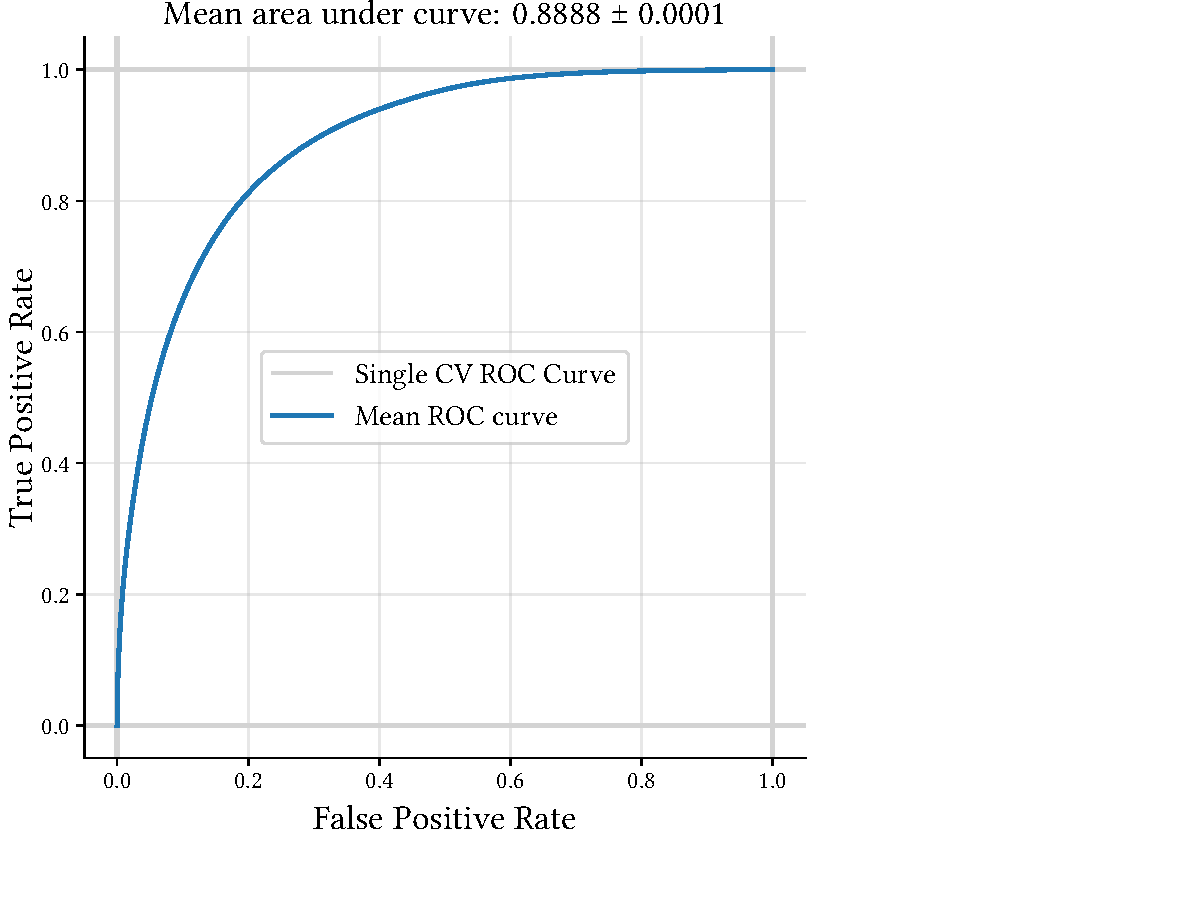
\includegraphics[page=1, width=.8\textwidth]{../analysis/plots/cross_val_sep_perf_plot.pdf}
    \caption{ROC-curve for the gamma/hadron separation on the cross validated training set 
    consisting of \num{6035652} proton events and \num{5753708} diffuse gamma events in total.
    The five ROC-curves from the individual cross validation steps show almost no deviation.}
    \label{fig:gh_roc}
\end{figure}


The feature importance, as calculated via sklearn, is shown in figure \ref{fig:gh_features}.
\begin{figure}
    \centering
    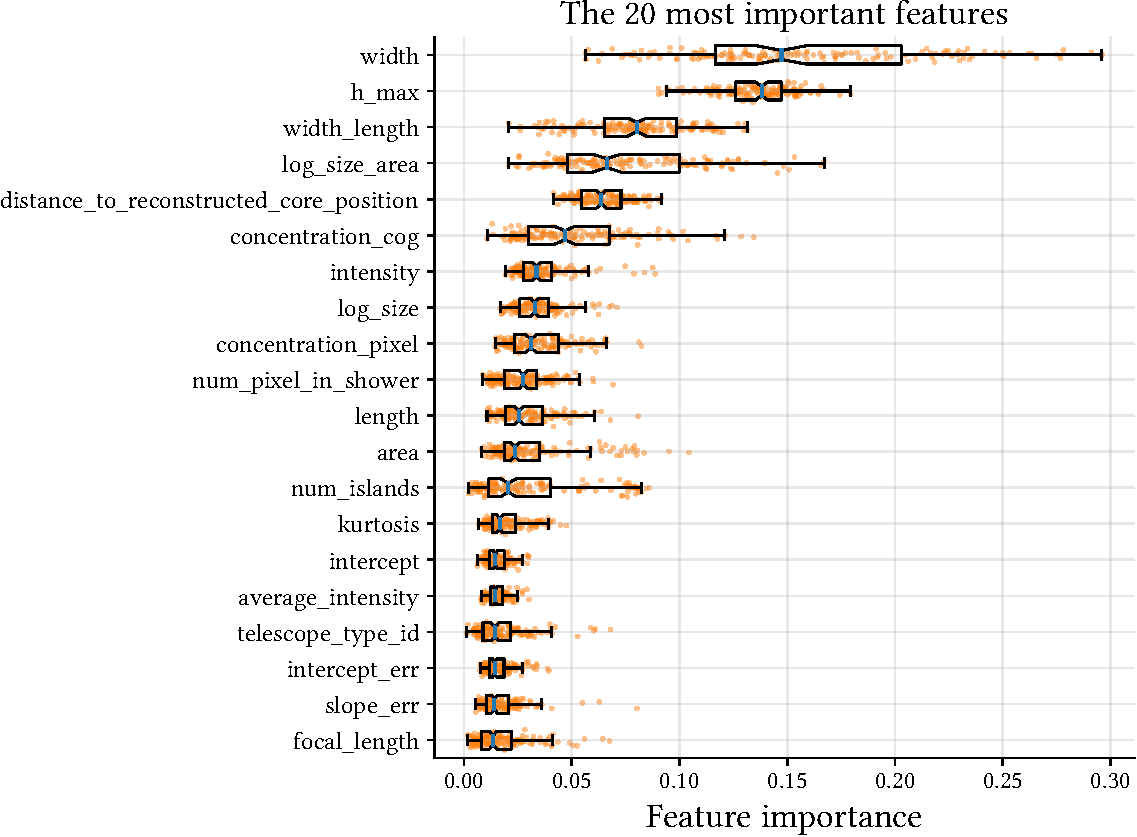
\includegraphics[page=1, width=.8\textwidth]{../analysis/plots/separation_features.pdf}
    \caption{Feature importance for the gamma/hadron separation.}
    \label{fig:gh_features}
\end{figure}


The resulting precision, recall and $f$-score are shown in figure \ref{fig:gh_fscore}.

\begin{figure}
    \centering
    \includegraphics[page=3, width=.8\textwidth]{../analysis/plots/cross_val_sep_perf_plot.pdf}
    \caption{Precision, recall and F-score for the gamma/hadron separation model on the 
    cross-validated dataset. The maximum F-score is achieved at a prediction threshold
    of $\approx \num{0.82}$.}
    \label{fig:gh_fscore}
\end{figure}

For the hadroness cut, that we apply later, we will choose the maximum of the $f_{\num{0.1}}$-score
at $\approx \num{0.82}$